\subsection{Perdita di energia e angolo}   % titolo provvisorio

\marginpar{L'incipit non è dei migliori, ma io non so dove sarà questo pezzo a relazione finita e faccio il possibile}
La perdita di energia di una particella carica all'interno di un materiale dipende anche dalla distanza percorsa in esso. Nel nostro caso è l'angolo di incidenza a stabilire quanta strada farà un muone nella lastra di scintillatore plastico. Per valutare l'entità di questo effetto abbiamo operato nel seguente modo: sfruttando l'ADC misuriamo l'energia persa nell'attraversare la lastra del PM6 selezionando particelle che incidono a grande angolo oppure a piccolo angolo.
Per selezionare le particelle a piccolo angolo misuriamo le coincidenze PM1 \& PM6, per fare l'opposto contiamo le particelle che soddisfano la configurazione PM6 \& PM5 $\neg$ PM4.
\marginpar{Figura provvisoria. Indovina indovinello chi farà quel disegnello?}
La \autoref{ang} illustra la strategia di misura. Ci aspettiamo che le particelle che incidono con angolo maggiore perdano più energia, quindi la loro distribuzione di Landau  ha una moda spostata più a destra.

\begin{figure}[h]
\centering
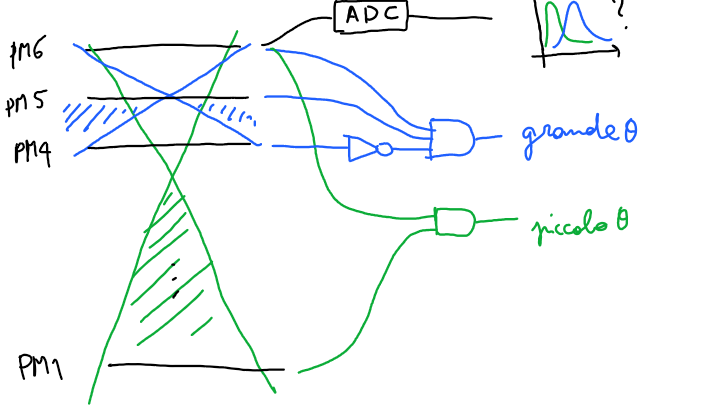
\includegraphics[width=8 cm]{ang}
\caption{schema della strategia di coincidenze per selezionare l'angolo delle particelle incidenti.}
\label{ang}
\end{figure}

Questo è ciò che abbiamo effettivamente verificato. Infatti la moda per la distribuzione a grande angolo è $M_\theta=\SI{307\pm7}{mV}$, mentre quella per angoli piccoli vale $m_\theta=\SI{250\pm5}{mV}$. In \autoref{isto} sono presenti gli istogrammi ottenuti dalle due configurazioni di misura.
\marginpar{l'errore è la semilarghezza del bin}
\begin{figure}[h]
\centering
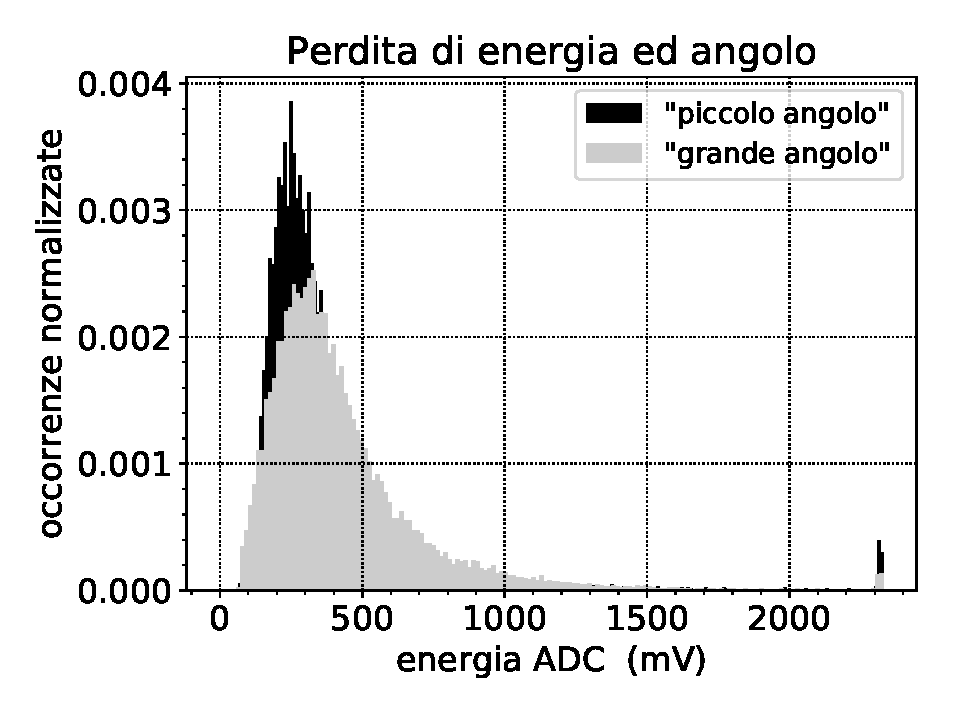
\includegraphics[width=8 cm]{angoli}
\caption{istogrammi relativi alle distribuzioni angolari dei muoni. Il picco presente sulla coda è causato dagli eventi abbastanza energetici da saturare l'uscita dell'amplificatore.}
\label{isto}
\end{figure}
